
%% 
%% Copyright 2007, 2008, 2009 Elsevier Ltd
%% 
%% This file is part of the 'Elsarticle Bundle'.
%% ---------------------------------------------
%% 
%% It may be distributed under the conditions of the LaTeX Project Public
%% License, either version 1.2 of this license or (at your option) any
%% later version.  The latest version of this license is in
%%    http://www.latex-project.org/lppl.txt
%% and version 1.2 or later is part of all distributions of LaTeX
%% version 1999/12/01 or later.
%% 
%% The list of all files belonging to the 'Elsarticle Bundle' is
%% given in the file `manifest.txt'.
%% 

%% Template article for Elsevier's document class `elsarticle'
%% with numbered style bibliographic references
%% SP 2008/03/01

%\documentclass[preprint,12pt]{elsarticle}

%% Use the option review to obtain double line spacing
%% \documentclass[authoryear,preprint,review,12pt]{elsarticle}

%% Use the options 1p,twocolumn; 3p; 3p,twocolumn; 5p; or 5p,twocolumn
%% for a journal layout:
%%\documentclass[final,1p,times]{elsarticle}
%\documentclass[final,1p,times,twocolumn]{elsarticle}
%% \documentclass[final,3p,times]{elsarticle}
%% \documentclass[final,3p,times,twocolumn]{elsarticle}
%% \documentclass[final,5p,times]{elsarticle}
 \documentclass[final,5p,times,twocolumn]{elsarticle}

%% For including figures, graphicx.sty has been loaded in
%% elsarticle.cls. If you prefer to use the old commands
%% please give \usepackage{epsfig}

%% The amssymb package provides various useful mathematical symbols
\usepackage{amssymb}
\usepackage{check-short}
\usepackage{overpic}
\usepackage{multirow}
%\usepackage{enumerate}

%% The lineno packages adds line numbers. Start line numbering with
%% \begin{linenumbers}, end it with \end{linenumbers}. Or switch it on
%% for the whole article with \linenumbers.
%% \usepackage{lineno}


\begin{document}
\pagestyle{empty}

\newlength{\fwd}
\newlength{\fht}


\fwd = .4\textwidth
\fht = .1\textheight	
\begin{figure*}[]
	{
	\small
	% \begin{tabular}{p{\fwd} p{\fwd}}
	\begin{tabular}{c c}
		% This file was created by matlab2tikz.
%
%The latest updates can be retrieved from
%  http://www.mathworks.com/matlabcentral/fileexchange/22022-matlab2tikz-matlab2tikz
%where you can also make suggestions and rate matlab2tikz.
%
\definecolor{mycolor1}{rgb}{0.00000,0.44700,0.74100}%
\definecolor{mycolor2}{rgb}{0.85000,0.32500,0.09800}%
%
\begin{tikzpicture}

\begin{axis}[%
width=0.951\fwd,
height=0.75\fht,
at={(0\fwd,0\fwd)},
scale only axis,
xmin=0,
xmax=40,
xlabel={time [s]},
ymin=0,
ymax=2.5e-07,
ylabel={$C$ $\text{[mmol/mm}^\text{3}\text{]}$},
axis background/.style={fill=white},
legend style={legend cell align=left,align=left,draw=white!15!black}
]
\addplot [color=mycolor1,solid,very thick]
  table[row sep=crcr]{%
0	0\\
0.4	0\\
0.8	0\\
1.2	0\\
1.6	0\\
2	5.62373487759478e-11\\
2.4	1.09810271021085e-09\\
2.8	6.76053034703798e-09\\
3.2	2.13478347753626e-08\\
3.6	4.56056649657982e-08\\
4	7.67693039618778e-08\\
4.4	1.10760368816952e-07\\
4.8	1.43746597983364e-07\\
5.2	1.72821999990385e-07\\
5.6	1.96160012105964e-07\\
6	2.12907090713985e-07\\
6.4	2.22973323725445e-07\\
6.8	2.26804741960865e-07\\
7.2	2.25178885025859e-07\\
7.6	2.19040032343215e-07\\
8	2.09376955393214e-07\\
8.4	1.97139176006753e-07\\
8.8	1.83184972235038e-07\\
9.2	1.6825381701405e-07\\
9.6	1.5295649926078e-07\\
10	1.3777726549853e-07\\
10.4	1.23083485704354e-07\\
10.8	1.09139475580703e-07\\
11.2	9.61220627108628e-08\\
11.6	8.41362598740187e-08\\
12	7.32300105168483e-08\\
12.4	6.34074188236187e-08\\
12.8	5.46401838538925e-08\\
13.2	4.68771886140848e-08\\
13.6	4.00523095626387e-08\\
14	3.4090617904463e-08\\
14.4	2.89131601344388e-08\\
14.8	2.44405364930844e-08\\
15.2	2.05954798314946e-08\\
15.6	1.73046252038486e-08\\
16	1.44996421001143e-08\\
16.4	1.21178699857602e-08\\
16.8	1.01025854633713e-08\\
17.2	8.40299542178553e-09\\
17.6	6.97404198461131e-09\\
18	5.77607935091924e-09\\
18.4	4.77447355834304e-09\\
18.8	3.93916172160292e-09\\
19.2	3.24419737926786e-09\\
19.6	2.66730266166506e-09\\
20	2.18943870651418e-09\\
20.4	1.79440465920876e-09\\
20.8	1.46846847064005e-09\\
21.2	1.20003289411346e-09\\
21.6	9.79336326007395e-10\\
22	7.98187748378252e-10\\
22.4	6.49733970754416e-10\\
22.8	5.28256526672998e-10\\
23.2	4.28995952016572e-10\\
23.6	3.48000282397405e-10\\
24	2.81995444125054e-10\\
24.4	2.28274651883307e-10\\
24.8	1.84604584011355e-10\\
25.2	1.49146036254608e-10\\
25.6	1.20387064957272e-10\\
26	9.70868785116934e-11\\
26.4	7.82288318545415e-11\\
26.8	6.29812300119354e-11\\
27.2	5.06646643040334e-11\\
27.6	4.07249116439323e-11\\
28	3.27104678363883e-11\\
28.4	2.62539803586422e-11\\
28.8	2.10569311946487e-11\\
29.2	1.68770204325555e-11\\
29.6	1.35178038053597e-11\\
30	1.0820183236205e-11\\
30.4	8.65544366249652e-12\\
30.8	6.91955310729552e-12\\
31.2	5.5285112362483e-12\\
31.6	4.41455486319452e-12\\
32	3.52306811834916e-12\\
32.4	2.81007005409287e-12\\
32.8	2.2401727856489e-12\\
33.2	1.78492607969931e-12\\
33.6	1.42147458549083e-12\\
34	1.13147177733343e-12\\
34.4	0\\
34.8	0\\
35.2	0\\
35.6	0\\
36	0\\
36.4	0\\
36.8	0\\
37.2	0\\
37.6	0\\
38	0\\
38.4	0\\
38.8	0\\
39.2	0\\
39.6	0\\
};
\addlegendentry{Convolution};

\addplot [color=mycolor2,dashed,very thick]
  table[row sep=crcr]{%
0	0\\
0.4	0\\
0.8	0\\
1.2	0\\
1.6	0\\
2	5.3279568073074e-11\\
2.4	1.07821521955639e-09\\
2.8	6.71290754043026e-09\\
3.2	2.12564956013061e-08\\
3.6	4.54228810841506e-08\\
4	7.64315332182225e-08\\
4.4	1.10213523840219e-07\\
4.8	1.42958770768866e-07\\
5.2	1.71785826132747e-07\\
5.6	1.94889508729946e-07\\
6	2.11432221500284e-07\\
6.4	2.21334146149828e-07\\
6.8	2.25046160287466e-07\\
7.2	2.23346407714781e-07\\
7.6	2.17176667633836e-07\\
8	2.07521150089304e-07\\
8.4	1.95323644243314e-07\\
8.8	1.81436224500391e-07\\
9.2	1.66592199968555e-07\\
9.6	1.51396589797636e-07\\
10	1.3632847936435e-07\\
10.4	1.21750799207446e-07\\
10.8	1.07924182119412e-07\\
11.2	9.50225094085739e-08\\
11.6	8.31485298722586e-08\\
12	7.2348531031234e-08\\
12.4	6.26254832899861e-08\\
12.8	5.39503908539349e-08\\
13.2	4.62717953679953e-08\\
13.6	3.95235135517039e-08\\
14	3.36307690244454e-08\\
14.4	2.85149175130422e-08\\
14.8	2.40969765219252e-08\\
15.2	2.03001649700339e-08\\
15.6	1.70516423039829e-08\\
16	1.4283615166056e-08\\
16.4	1.19339562230449e-08\\
16.8	9.94645645486966e-09\\
17.2	8.27081040255549e-09\\
17.6	6.86241431416851e-09\\
18	5.68204011719055e-09\\
18.4	4.6954337247387e-09\\
18.8	3.87287421966553e-09\\
19.2	3.18872072804604e-09\\
19.6	2.62096602035629e-09\\
20	2.15080978220791e-09\\
20.4	1.76225980427895e-09\\
20.8	1.44176580276721e-09\\
21.2	1.17788797530892e-09\\
21.6	9.61000531233148e-10\\
22	7.83029147436785e-10\\
22.4	6.37220457950388e-10\\
22.8	5.1794117711445e-10\\
23.2	4.20504195487211e-10\\
23.6	3.41018904827157e-10\\
24	2.76263049750932e-10\\
24.4	2.23573527582697e-10\\
24.8	1.80753733306562e-10\\
25.2	1.45995250370183e-10\\
25.6	1.17811903729239e-10\\
26	9.4984407302507e-11\\
26.4	7.65140460587736e-11\\
26.8	6.15840282729948e-11\\
27.2	4.95273231768238e-11\\
27.6	3.97999619242864e-11\\
28	3.19589252105288e-11\\
28.4	2.56438694661132e-11\\
28.8	2.05620562202835e-11\\
29.2	1.64759471844691e-11\\
29.6	1.31930121953556e-11\\
30	1.05573697632337e-11\\
30.4	8.44294196192858e-12\\
30.8	6.74785807138353e-12\\
31.2	5.38988595036491e-12\\
31.6	4.30270767561291e-12\\
32	3.43288752398976e-12\\
32.4	2.73740677349094e-12\\
32.8	2.18166182862043e-12\\
33.2	1.73784050750156e-12\\
33.6	1.38360654329319e-12\\
34	1.10103495034139e-12\\
34.4	0\\
34.8	0\\
35.2	0\\
35.6	0\\
36	0\\
36.4	0\\
36.8	0\\
37.2	0\\
37.6	0\\
38	0\\
38.4	0\\
38.8	0\\
39.2	0\\
39.6	0\\
};
\addlegendentry{PDE};

\end{axis}
\end{tikzpicture}% & \input{./figs/IDecVSIAna.tikz}\\
	\end{tabular}
	}
	\caption{}
	\label{fig:VoxelCompFIG}
\end{figure*}
\clearpage

	\begin{figure*}[]
	    \centering
	    \begin{overpic}[scale=0.3]{figs/perfusion-problem.eps}
	    	\put(10,70){\color{black}$F_0$}
			\put(48,70){\color{black}$F_0$}
			\put(84,70){\color{black}$\Delta F_0$}
			\put(10,33){\color{black}$2V$}
			\put(49,20){\color{black}$V$}
			\put(49,45){\color{black}$V$}
			\put(91,42){\color{black}$\Delta V$}
		\end{overpic}
	    \caption*{}
	    \label{fig:perfusion-problemFIG}
	\end{figure*}
\clearpage

\begin{figure*}[]
	\centering
	\fwd = .23\textwidth
	\begin{tabular}{c c c c}
		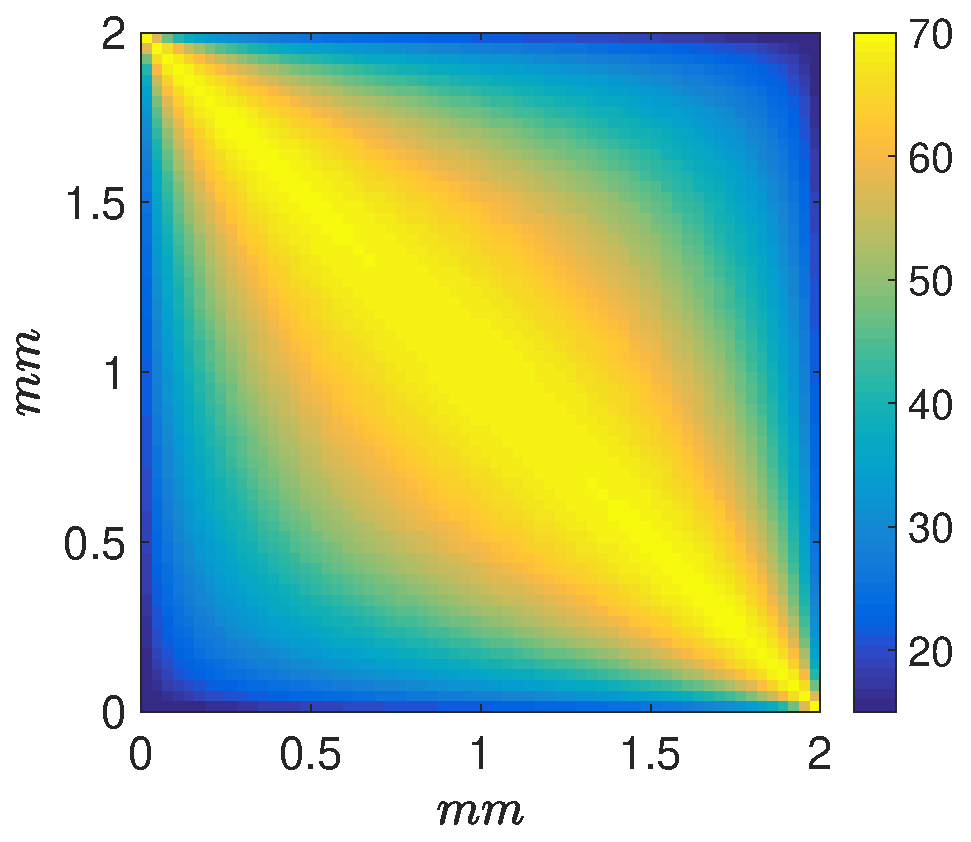
\includegraphics[width=\fwd]{figs/E110_CBFOnDifferentResolutions_plot-Ps-scaleto-none-raw.eps} 
		& 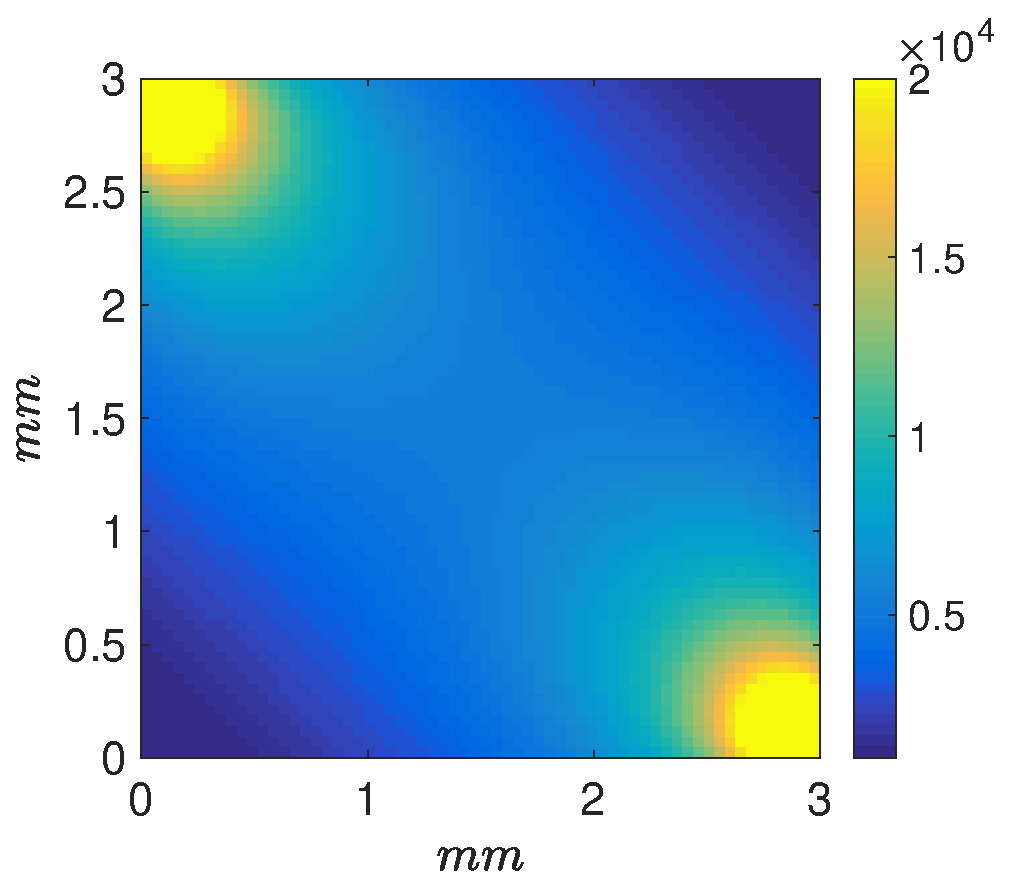
\includegraphics[width=\fwd]{figs/E110_CBFOnDifferentResolutions_plot-Pv-scaleto-none-raw.eps}
		& \includegraphics[width=\fwd]{figs/E110_CBFOnDifferentResolutions_plot-bSVD-scaleto-none-raw.eps}
		& \includegraphics[width=\fwd]{figs/E110_CBFOnDifferentResolutions_plot-MS-scaleto-none-raw.eps}\\
		(a) $P_{\mathrm{s}}(\mathbf{x})$. & (b) $P_{\mathrm{v}}(\mathbf{x})$ & (c) $P_{\mathrm{bSVD}}(\mathbf{x})$. & (d) $P_{\mathrm{MS}}(\mathbf{x})$.
	\end{tabular}
	\caption*{} 
        \label{fig:perfusionmapsFIG}
\end{figure*}	
\clearpage

    \begin{figure*}[]
    	\centering
    	\fwd = .46\textwidth
    	\begin{tabular}{c c}
    		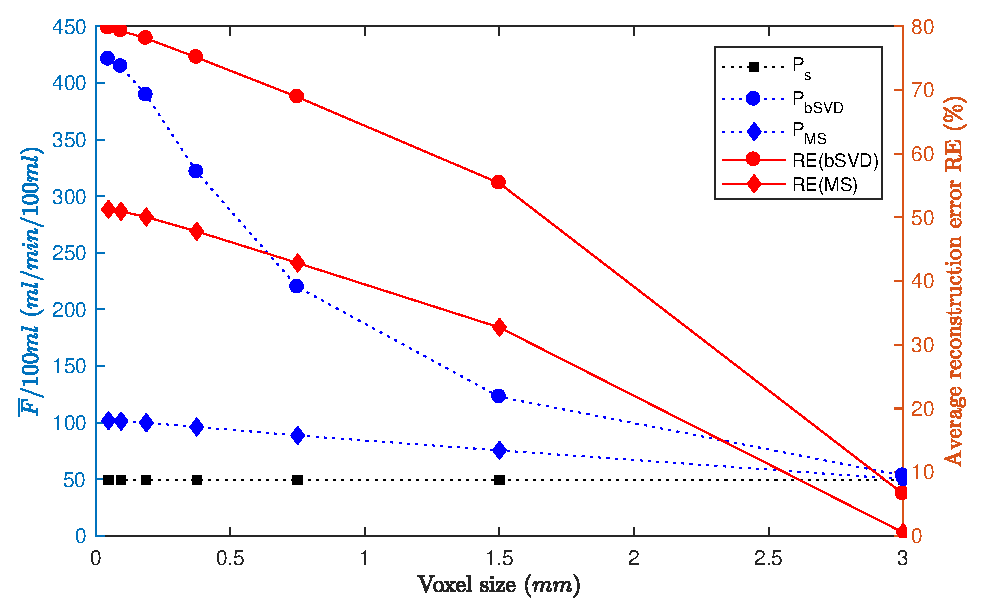
\includegraphics[width=\fwd]{figs/E110_CBFOnDifferentResolutions_plot-Ps-scaleto-none.eps} & 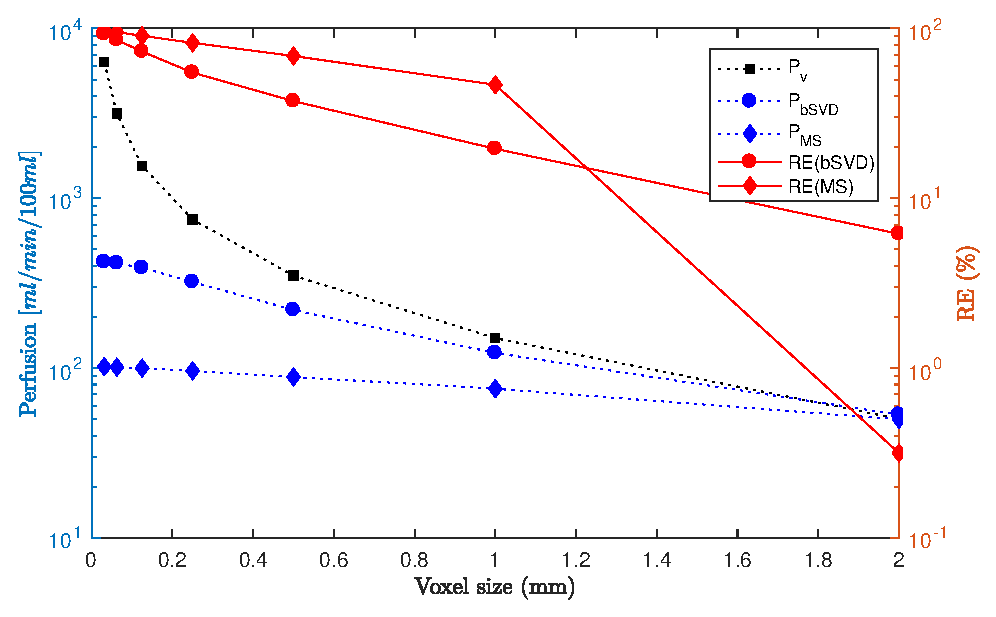
\includegraphics[width=\fwd]{figs/E110_CBFOnDifferentResolutions_plot-Pv-scaleto-none.eps}\\	
    		(a) Comparison to global perfusion $P_{\mathrm{s}}$. & (b) Comparison to local perfusion $P_{\mathrm{v}}$. \\
    	\end{tabular}
    	\caption*{}
            \label{fig:volnormperfFIG}
    \end{figure*}
\clearpage

    \begin{figure*}[]
    	\centering
    	\fwd = .46\textwidth
    	\begin{tabular}{c c}
    		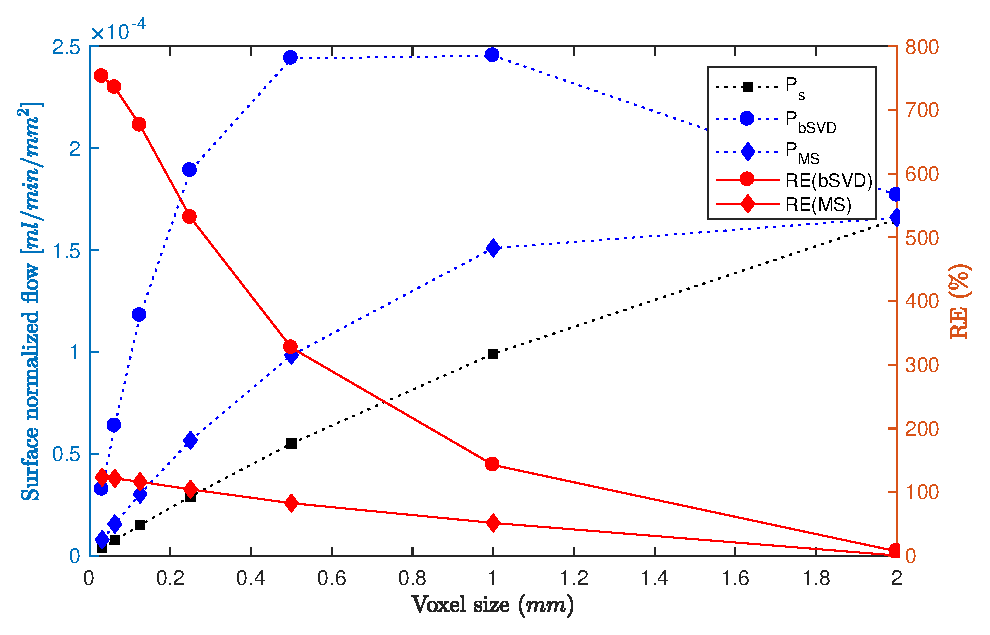
\includegraphics[width=\fwd]{figs/E110_CBFOnDifferentResolutions_plot-Ps-scaleto-S.eps} & 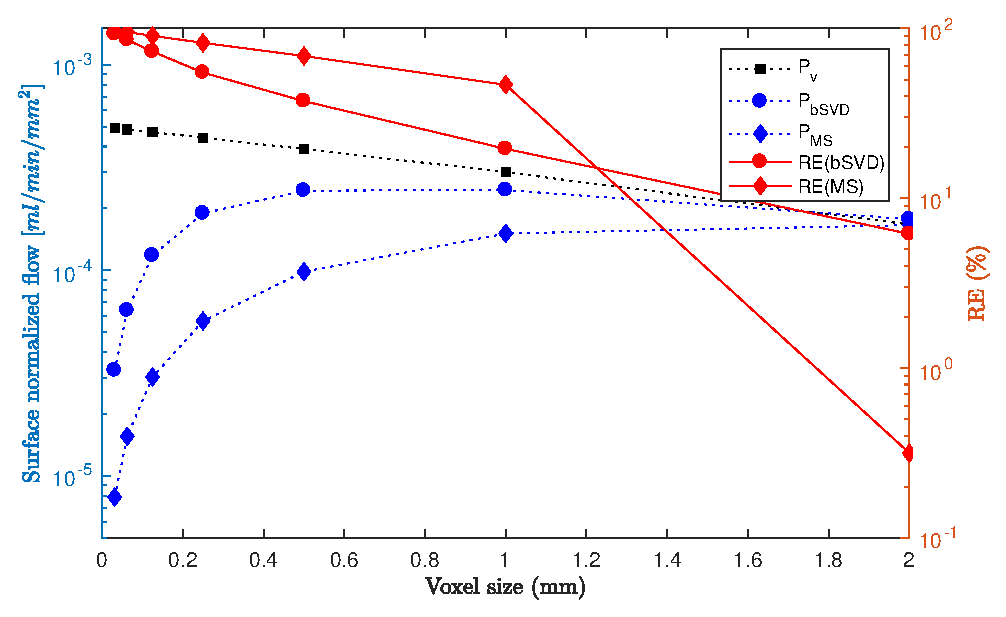
\includegraphics[width=\fwd]{figs/E110_CBFOnDifferentResolutions_plot-Pv-scaleto-S.eps}\\	
    		(a) Comparison to global perfusion $P_{\mathrm{s}}$. & (b) Comparison to local perfusion $P_{\mathrm{v}}$.
    	\end{tabular}
    	\caption*{}
            \label{fig:surfnormperfFIG}
    \end{figure*}
\clearpage

	\begin{figure*}[]
		\fwd = .21\textwidth
		\centering
		\begin{tabular}{ccc}
		 {\small% This file was created by matlab2tikz.
%
%The latest updates can be retrieved from
%  http://www.mathworks.com/matlabcentral/fileexchange/22022-matlab2tikz-matlab2tikz
%where you can also make suggestions and rate matlab2tikz.
%
\definecolor{mycolor1}{rgb}{0.00000,0.44700,0.74100}%
%
\begin{tikzpicture}

\begin{axis}[%
width=0.951\fwd,
height=0.75\fwd,
at={(0\fwd,0\fwd)},
scale only axis,
xmin=0,
xmax=120,
xlabel={time [s]},
ymin=0,
ymax=250,
ylabel={rel. concentration},
axis background/.style={fill=white}
]
\addplot [color=mycolor1,solid,forget plot,thick]
  table[row sep=crcr]{%
0	0\\
5	4.81948215980018\\
10	11.7249407767123\\
15	109.788176034815\\
20	221.037522824365\\
25	141.890221064755\\
30	49.1060473080009\\
35	27.7167012296253\\
40	34.5042336994668\\
45	46.9343027309933\\
50	38.6517774527303\\
55	37.0988211659761\\
60	37.9793720995833\\
65	38.8599230331905\\
70	39.7404739667976\\
75	40.6210249004048\\
80	41.501575834012\\
85	42.3663391649169\\
90	41.668129828291\\
95	40.969920491665\\
100	40.2717111550391\\
105	39.5735018184132\\
110	38.8752924817873\\
};
\end{axis}
\end{tikzpicture}%} & \includegraphics[width = \fwd]{./figs/real_axial160.pdf} & {\small% This file was created by matlab2tikz.
%
%The latest updates can be retrieved from
%  http://www.mathworks.com/matlabcentral/fileexchange/22022-matlab2tikz-matlab2tikz
%where you can also make suggestions and rate matlab2tikz.
%
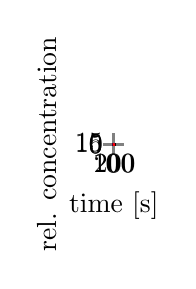
\begin{tikzpicture}

\begin{axis}[%
width=0.951\fwd,
height=0.75\fwd,
at={(0\fwd,0\fwd)},
scale only axis,
xmin=0,
xmax=250,
xlabel={time [s]},
ymin=-2,
ymax=14,
ylabel={rel. concentration},
axis background/.style={fill=white}
]
\addplot [color=blue,solid,forget plot,thick]
  table[row sep=crcr]{%
0	0\\
5.10888888888889	3.57728482303029\\
10.2177777777778	3.8501111093967\\
15.3266666666667	5.71664126840386\\
20.4355555555556	10.3940019898786\\
25.5444444444444	13.3104878781745\\
30.6533333333333	9.7857007250912\\
35.7622222222222	7.15008816358801\\
40.8711111111111	6.69575791027159\\
45.98	7.0175162477114\\
51.0888888888889	7.11075546536433\\
56.1977777777778	7.06466948033182\\
61.3066666666667	7.08320213588359\\
66.4155555555556	7.1017347914334\\
71.5244444444444	7.12026744698453\\
76.6333333333333	7.13880010253569\\
81.7422222222222	7.15733275808708\\
86.8511111111111	7.17427131128685\\
91.96	7.03339373168847\\
97.0688888888889	6.89251615209099\\
102.177777777778	6.75163857249418\\
107.286666666667	6.61076099289567\\
112.395555555556	6.46988341329856\\
117.504444444444	0\\
122.613333333333	0\\
127.722222222222	0\\
132.831111111111	0\\
137.94	0\\
143.048888888889	0\\
148.157777777778	0\\
153.266666666667	0\\
158.375555555556	0\\
163.484444444444	0\\
168.593333333333	0\\
173.702222222222	0\\
178.811111111111	0\\
183.92	0\\
189.028888888889	0\\
194.137777777778	0\\
199.246666666667	0\\
204.355555555556	0\\
209.464444444444	0\\
214.573333333333	0\\
219.682222222222	0\\
224.791111111111	0\\
229.9	0\\
};
\addplot [color=red,solid,forget plot,thick]
  table[row sep=crcr]{%
0	0.242877310049657\\
5.10888888888889	3.27801404634268\\
10.2177777777778	4.19212893178922\\
15.3266666666667	5.35931224793637\\
20.4355555555556	10.7296350477088\\
25.5444444444444	13.0351453456191\\
30.6533333333333	9.97028747702823\\
35.7622222222222	7.06991667403901\\
40.8711111111111	6.67958740784569\\
45.98	7.10086370332965\\
51.0888888888889	7.00395379245554\\
56.1977777777778	7.14771381111792\\
61.3066666666667	7.0617592832064\\
66.4155555555556	7.04431690009689\\
71.5244444444444	7.24681150319147\\
76.6333333333333	6.97944442254963\\
81.7422222222222	7.29409620580436\\
86.8511111111111	7.12166516958014\\
91.96	6.94933713547804\\
97.0688888888889	7.14300746526767\\
102.177777777778	6.3362801703634\\
107.286666666667	7.15680159666211\\
112.395555555556	5.8535182522262\\
117.504444444444	0.612745947271016\\
122.613333333333	-0.537195282539902\\
127.722222222222	0.406490463075758\\
132.831111111111	-0.24779589623344\\
137.94	0.091958881285865\\
143.048888888889	0.0337330911498852\\
148.157777777778	-0.111471653403876\\
153.266666666667	0.136091537098496\\
158.375555555556	-0.114848569476664\\
163.484444444444	0.0641204450664707\\
168.593333333333	-0.00415036164469126\\
173.702222222222	-0.0465858173026518\\
178.811111111111	0.0758150018721239\\
183.92	-0.0795846098022592\\
189.028888888889	0.061693871067431\\
194.137777777778	-0.0308886810616511\\
199.246666666667	-0.00308806028012709\\
204.355555555556	0.0332184262864778\\
209.464444444444	-0.0574855553444383\\
214.573333333333	0.0790144471363498\\
219.682222222222	-0.104119919783985\\
224.791111111111	0.139008058015951\\
229.9	-0.186333192218881\\
};
\end{axis}
\end{tikzpicture}%} \\
		 (a) & (b) & (c) 
		\end{tabular}
		\caption*{}
	\label{fig:RealDataFIG}
	\end{figure*}

\end{document}
